%UNIT 11: DAMPED AND UNDAMPED LINEAR SYSTEMS
%%%%%%%%%%%%%%%%%%%%%%%%%%%
%%%% Put the following at the top of each .tex file  %
\pagestyle{fancy}
\renewcommand{\theUnit}{11}
\ifthenelse{\isundefined{\UnitPageNumbers}}{}{\setcounter{page}{1}}
\rhead{Unit \theUnit: Damped and Undamped Linear Systems}
\lhead{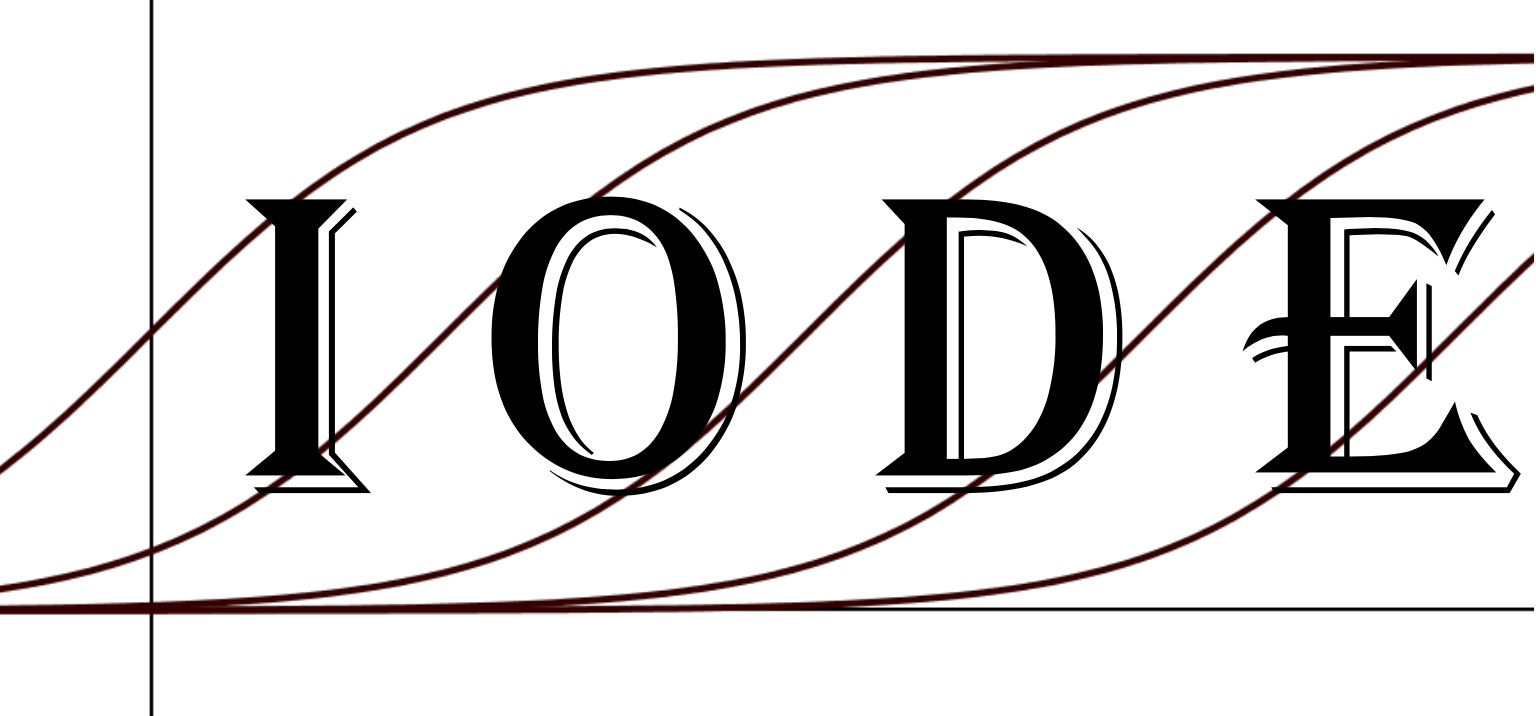
\includegraphics[width=1.25cm]{IODE-logo.png}}
\rfoot{\mypage}
\lfoot{}
\cfoot{}
\fancypagestyle{firstfooter}{\footskip = 50pt}
\renewcommand{\footrulewidth}{.4pt}
%%%%%%%%%%%%%%%%%%%%%%%%%%%
\vspace*{-20pt} \thispagestyle{firstfooter}
\pagebegin{Spiraling Solutions - Spring Mass Revisited}

In a previous problem we applied Newton's law of motion for a spring mass system and obtained the second order differential equation  $\displaystyle \frac{d^2x}{dt^2}+\frac{b}{m}\frac{dx}{dt}+\frac{k}{m}x=0$, where $x$ is the position of the object attached to the end of the spring, $m$ is the mass of the object, $b$ is the damping coefficient, and $k$ is the spring constant. Using the fact that velocity is the derivative of position and choosing the mass $m = 1$ and the spring constant $k = 2$, we converted this to the following system of two differential equations:  
\begin{center}
\raisebox{1.5\height}{$\displaystyle \begin{aligned}
\frac{dx}{dt}&=y \\ \frac{dy}{dt}&= -2x-by
\end{aligned}$} \hspace{1in}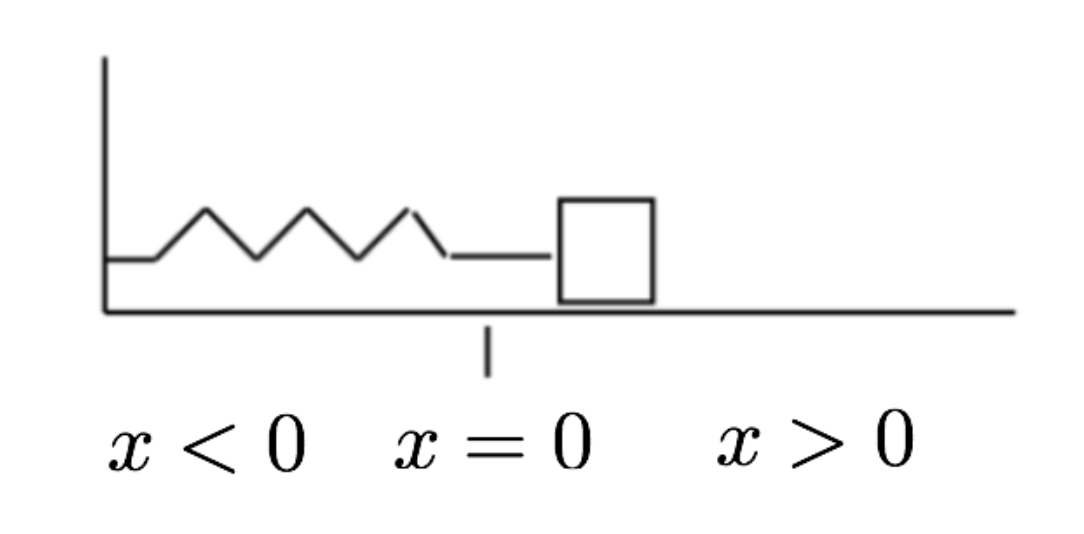
\includegraphics[width=2in]{11/11SpringMass.png}
\end{center}

We were able to figure out the $x(t)$ and $y(t)$ equations when the value of the friction parameter was such that there were straight line solutions in the phase plane. Such a situation is typically referred to as \textit{overdamped}. The situation is called \textit{damped} when the differential equations predict that the mass will oscillate about the 0 position and \textit{undamped} when there is no friction. In the following problems we figure out the $x(t)$ and $y(t)$ equations for the damped. We consider the undamped situation in the homework. \\

The vector field for the case when $b = 2$ is shown below. Based on this vector field, it appears that the differential equations predict that the mass will oscillate back and forth. Even though there are not any straight line solutions, we can still use the same algebraic approach as before to get the $x(t)$ and $y(t)$ equations for any initial condition, but we will have to deal complex numbers. Problems \ref{11problem1}-\ref{11problem7} outline a way to do this.
\begin{center}
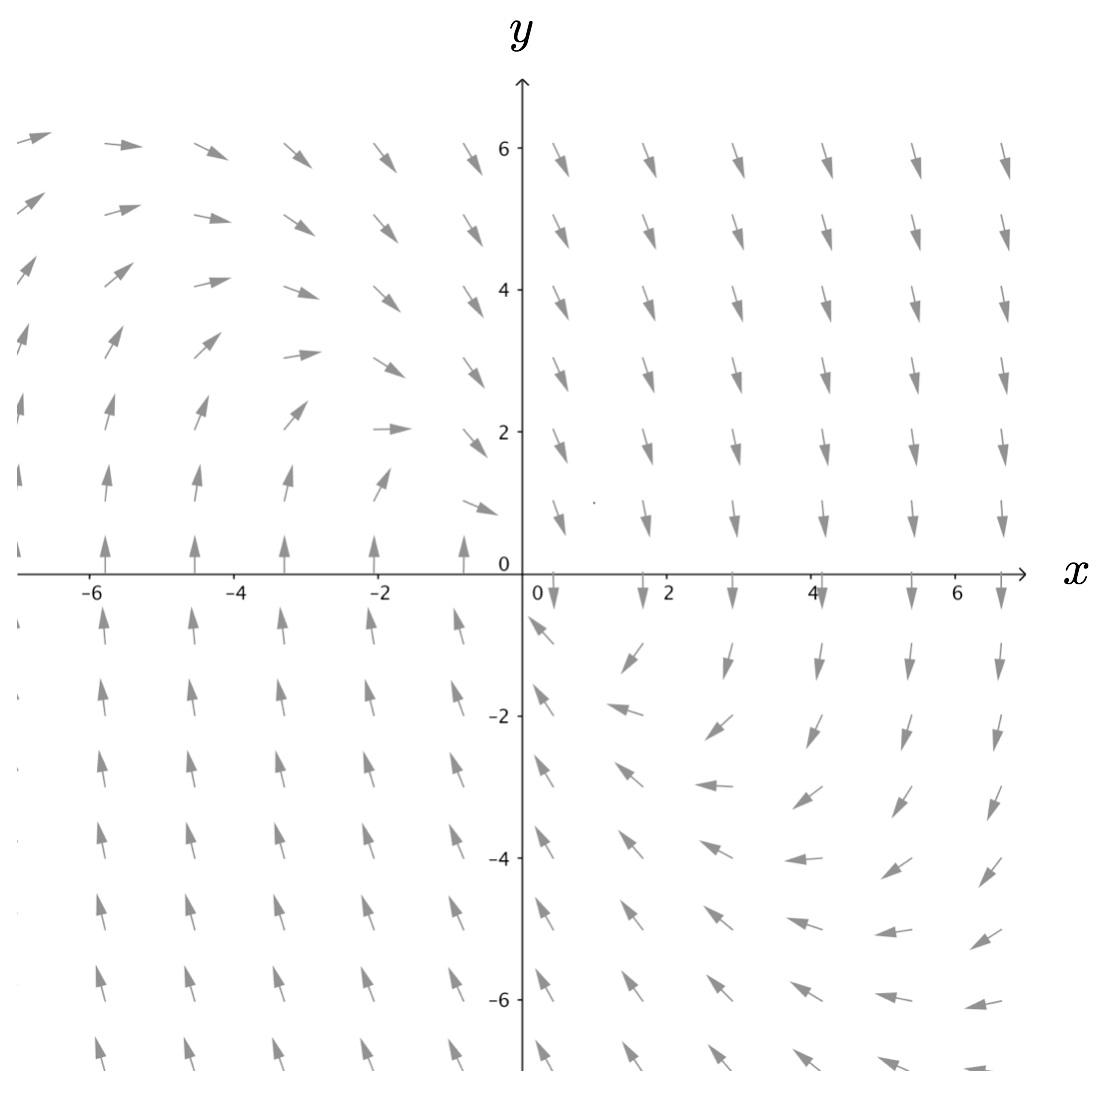
\includegraphics[width=3.5in]{11/11figure.png}
\end{center} 

\clearpage
\begin{enumerate}
\item	For the system of differential equations 
\begin{align*}
\frac{dx}{dt}&=y \\ \frac{dy}{dt}&= -2x-2y
\end{align*}
use the same algebraic approach as before to verify that the slopes of the ``straight line'' solutions are $-��1 \pm i$. \label{11problem1} \vfill

\item	For solutions with ``straight line'' slope $y=(-1+i)x$, find the $x(t)$ and $y(t)$ equations (in terms of complex numbers) for the solution along this ``straight line''�� with initial condition $(1, -1+i)$.\label{11problem2} \vfill

\clearpage

\item	For solutions with ``straight line'' slope  $y=(-1-i)x$, find the $x(t)$ and $y(t)$ equations (in terms of complex numbers) for the solution along this ``straight line'' with initial condition $(1, -1-i)$.\label{11problem3} \vfill

\item	Use Euler's formula $e^{a+ib}=e^ae^{ib}=e^a(\cos b+i\sin b)$ to rewrite the $x(t)$ and $y(t)$ equations from problem \ref{11problem2} (call these $x_1(t)$ and $y_1(t)$) and then again from problem \ref{11problem3} (call these $x_2(t)$ and $y_2(t)$). \label{11problem4} \vfill

\clearpage

\item	Denise suggests that if you add $\displaystyle \begin{pmatrix}
x_1(t)\\y_1(t)
\end{pmatrix}$ to $\displaystyle \begin{pmatrix}
x_2(t)\\y_2(t)
\end{pmatrix}$  the resulting pair of equations is (i) real valued and (ii) a solution to the same system of differential equations. Verify that this is true. \label{11problem5} \vfill

\item	Verify that if you subtract $\displaystyle \begin{pmatrix}
x_1(t)\\y_1(t)
\end{pmatrix}$  from $\displaystyle \begin{pmatrix}
x_2(t)\\y_2(t)
\end{pmatrix}$ and multiply the result by the complex number $i$, then the resulting pair of equations will be a real and a solution to the same system of differential equations. \label{11problem6} \vfill

\clearpage

\item	\label{11problem7}
\begin{enumerate}
\item Form the general solution to the system of differential equations 
\begin{align*}
\frac{dx}{dt}&=y \\ \frac{dy}{dt}&= -2x-2y
\end{align*}
\item What aspect of your general solution could be interpreted as the effect of friction on the spring mass system?
\item Find the particular solution for the initial condition (2, 3) and sketch the $x$ vs $t$ and $y$ vs $t$ graphs. 
\end{enumerate}
\end{enumerate}

\clearpage

%%%%%%%%%%%%%%%%%%%%%%%%%%%%%%%%%%%%%%%%%%%%%%
\pagebegin{Homework Set 11}

\begin{enumerate}
\item	The general solution to \label{11HWproblem1}
\begin{align*}
\frac{dx}{dt}&=y\\
\frac{dy}{dt}&= -2x-2y
\end{align*}
is
\begin{align*}
x(t) &= c_1e^{-t}\cos(t)+c_2e^{-t}\sin(t) \\
y(t) &= c_1e^{-t}(-\cos(t)-\sin(t))+c_2e^{-t}(-\sin(t)+\cos(t))
\end{align*}
Which part(s) of the general solution accounts for the fact that the differential equations predict that the mass will oscillate about the zero position? Which part(s) of the general solution accounts for the fact that the amplitude of the oscillations decreases over time?

\item	Suppose that for a different system of differential equations you got the exact same general solution as homework problem 1 except instead of $e^{-t}$ you got $e^t$. How would this change graphs of solutions in the phase plane? Explain. \label{11HWproblem2} 

\item	Find the general solution to the spring mass problem when there is no friction. Sketch these solution in the phase plane and explain how this general solution fits with your expectation for the behavior of the mass over time. Note: when there is no friction, $b = 0$, and the spring constant $k = 2$, we get \label{11HWproblem3}    
\begin{align*}
\frac{dx}{dt}&=y\\ \frac{dy}{dt}&= -2x
\end{align*}

\clearpage

\item Consider the phase planes below: \label{11HWproblem4} \\
\begin{enumerate*}
\item[(A)] 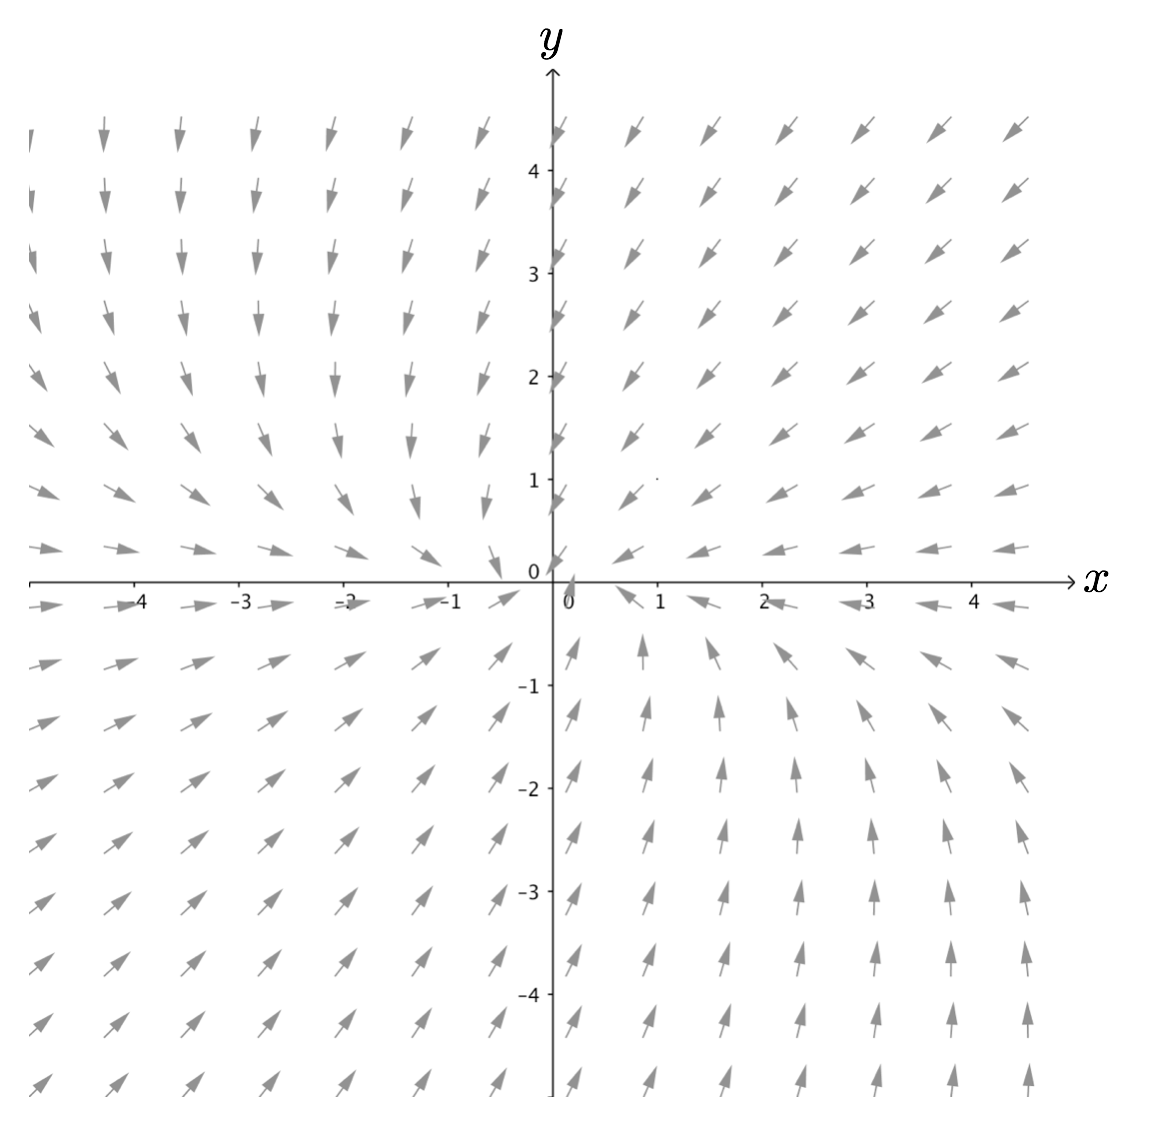
\includegraphics[width=2.5in]{11/11HWVectorField1.png}
\item[(B)] 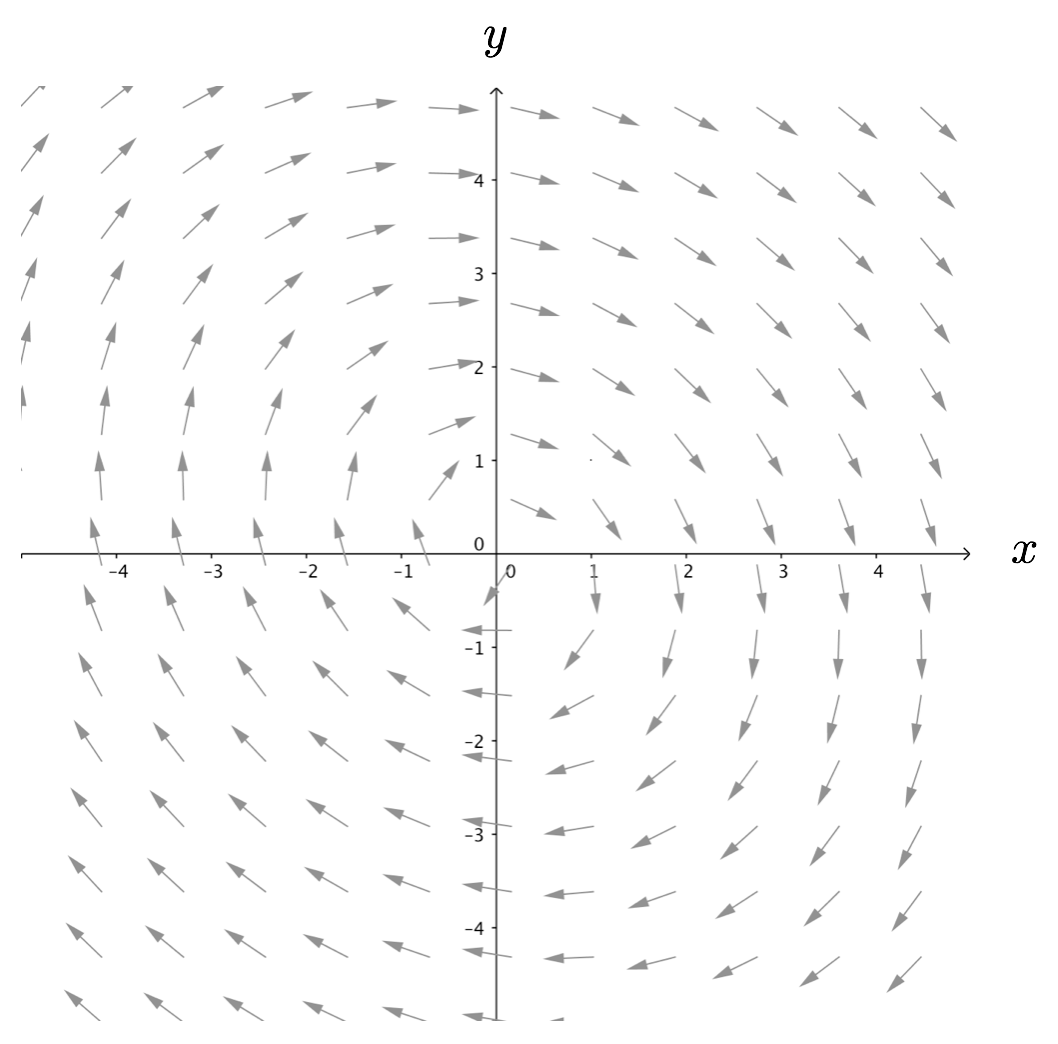
\includegraphics[width=2.5in]{11/11HWVectorField2.png} \\
\item[(C)] 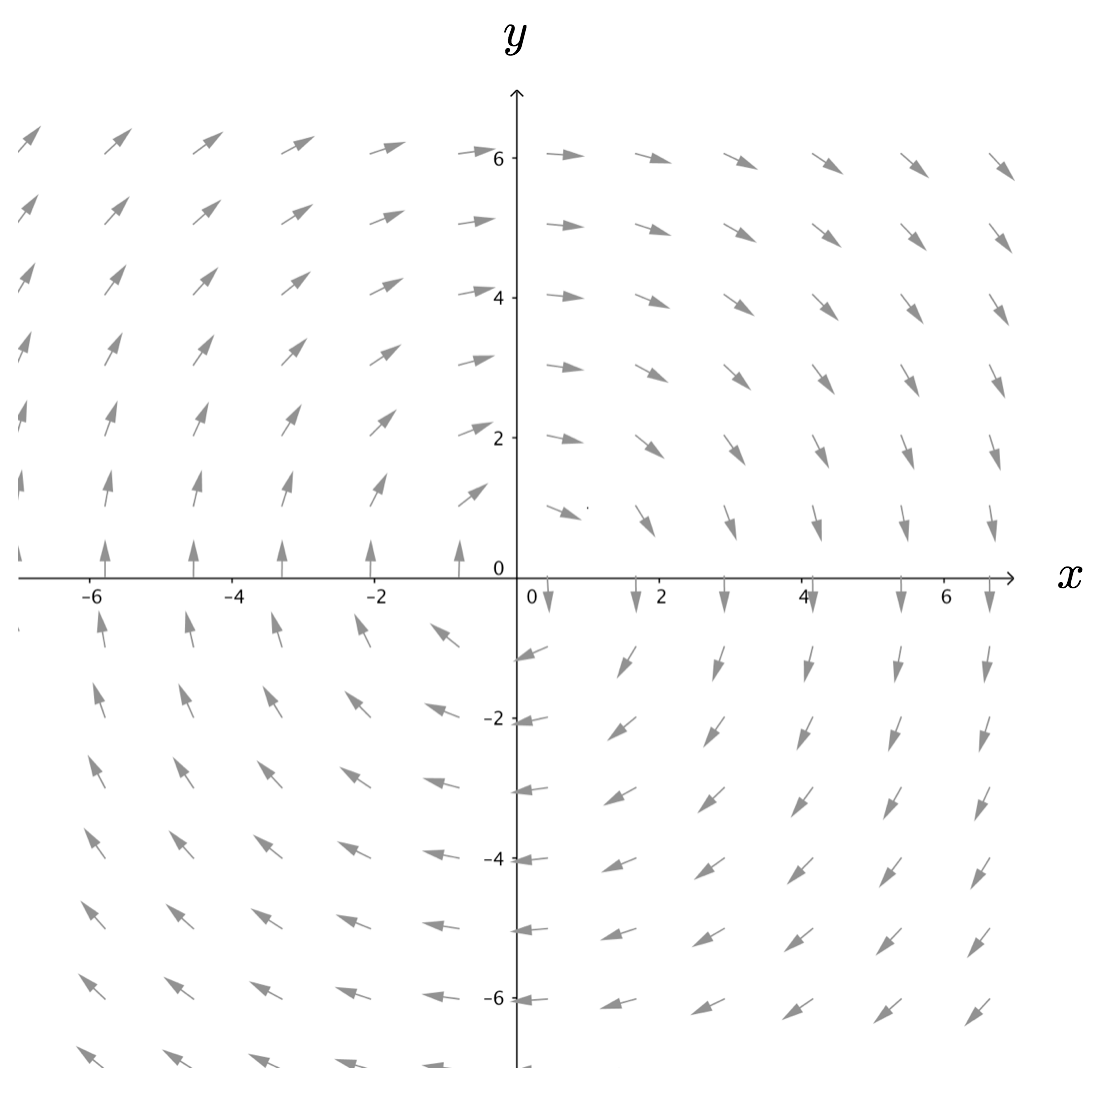
\includegraphics[width=2.5in]{11/11HWVectorField3.png}
\item[(D)] 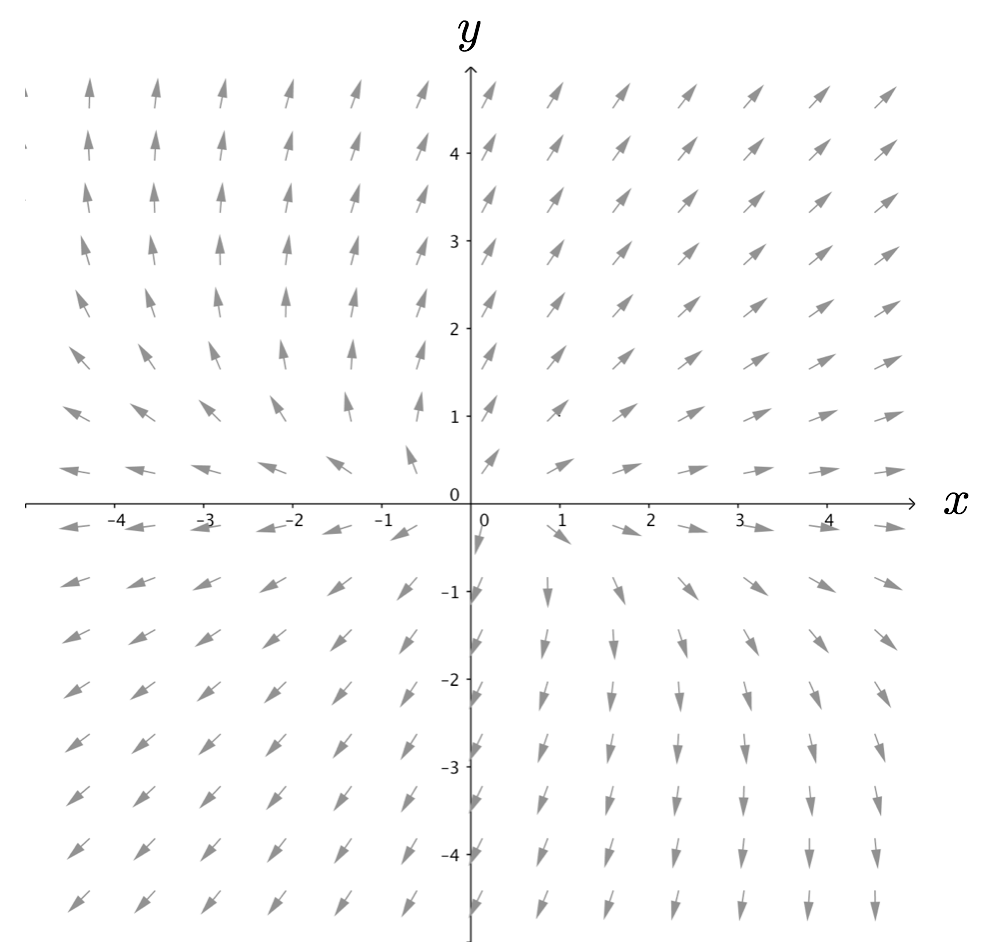
\includegraphics[width=2.5in]{11/11HWVectorField4.png}
\end{enumerate*}

For each sentence below, fill in the blank with choices from the following two lists:

\begin{center}
\begin{tabular}{ccccc}
\textbf{\underline{Spring System (First Blank)}} &&& \textbf{\underline{Solutions (Second Blank)}} \\
a damped spring &&& $c_1\cos(t) + c_2\sin(t)$ \\
an overdamped spring &&& $e^{-t}(c_1\cos(t) + c_2\sin(t))$ \\
an undamped spring &&& $e^{t}(c_1\cos(t) + c_2(\sin(t))$ \\
something other than a spring &&& $c_1 e^t + c_2 e^{2t}$ \\
&&& $c_1 e^{-t} + c_2 e^{-2t}$ \\
&&& $c_1 e^{-t} + c_2 e^{2t}$ \\
&&& $c_1 e^t + c_2 e^{-2t}$	
\end{tabular}
\end{center}

Phase plane (A) corresponds to \rule{1in}{.5pt} and the solutions look like $x(t)$=\rule{1.5in}{.5pt} \\

Phase plane (B) corresponds to \rule{1in}{.5pt} and the solutions look like $x(t)$=\rule{1.5in}{.5pt} \\

Phase plane (C) corresponds to \rule{1in}{.5pt} and the solutions look like $x(t)$=\rule{1.5in}{.5pt} \\

Phase plane (D) corresponds to \rule{1in}{.5pt} and the solutions look like $x(t)$=\rule{1.5in}{.5pt}

\clearpage

\item What type of system (undamped, damped, overdamped) do the following best correspond to? Explain your reasoning. \label{11HWproblem5}
\begin{enumerate}
\item A car that bounces every time it hits a bump
\item A pendulum immersed in a vat of honey
\item A bungee jumper
\end{enumerate}

\item In each part, write a differential equation corresponding to the given scenario: \label{11HWproblem6}
\begin{enumerate}
\item An undamped spring
\item An underdamped spring
\item An overdamped spring
\end{enumerate}

\item Does Adding Solutions Always Result in Another Solution? \\

In deriving the general solution to the spring mass problem, two solutions were added to get another solution. This worked for the particular equations at hand, but does adding two solutions to a system of differential equations of the form    
\begin{align*}
\frac{dx}{dt}&=ax+by\\ \frac{dy}{dt}&= cx+dy
\end{align*}
 always result in another solution to the same system of differential equations? Below is a proof that this in fact is true.

\noindent \underline{Claim}:
If  $\displaystyle \begin{pmatrix}
x_1(t)\\y_1(t)
\end{pmatrix}$  and $\displaystyle \begin{pmatrix}
x_2(t)\\y_2(t)
\end{pmatrix}$  are solutions (not necessarily straight line solutions) to a system of differential equations of the form  \begin{align*}\begin{split}
\frac{dx}{dt}&=ax+by\\ \frac{dy}{dt}&= cx+dy
\end{split}\end{align*}
 then the sum of these two solutions is also a solution. That is, if we call the sum of these two solutions  $\displaystyle \begin{pmatrix} x_3(t)\\y_3(t) \end{pmatrix}$ where 
 \[ \begin{pmatrix}
x_3(t)\\y_3(t)
\end{pmatrix}=\begin{pmatrix}
x_1(t)\\y_1(t)
\end{pmatrix}+\begin{pmatrix}
x_2(t)\\y_2(t)
\end{pmatrix}=\begin{pmatrix}
x_1(t)+x_2(t)\\y_1(t)+y_2(t)
\end{pmatrix},\]
 then  $\displaystyle \begin{pmatrix} x_3(t)\\y_3(t) \end{pmatrix}$  is also a solution to the same system of differential equations.  

\noindent\underline{Proof:}
In order to show that $\displaystyle \begin{pmatrix} x_3(t)\\y_3(t) \end{pmatrix}$  is a solution, we need to verify it satisfies the system of differential equations. This is, we need to show that  
\begin{align*}\begin{split}
\frac{d}{dt}x_3(t)&=ax_3(t)+by_3(t)\\ \frac{d}{dt}y_3(t)&= cx_3(t)+dy_3(t)
\end{split}.\end{align*}

Since   
\[ \begin{pmatrix}
x_3(t)\\y_3(t)\end{pmatrix}=\begin{pmatrix}
x_1(t)+x_2(t)\\y_1(t)+y_2(t)
\end{pmatrix},\] we know that   
\begin{align}\begin{split}
\frac{d}{dt}x_3(t)&=\frac{d}{dt}x_1(t)+\frac{d}{dt}x_2(t)\\ \frac{d}{dt}y_3(t)&= \frac{d}{dt}y_1(t)+\frac{d}{dt}y_2(t) 
\end{split}.\label{12HWeqn1}\end{align}
Because $\displaystyle \begin{pmatrix} x_1(t)\\y_1(t) \end{pmatrix}$   is a solution, it satisfies the system of differential equations. That is,    
\begin{align}\begin{split}
\frac{d}{dt}x_1(t)&=ax_1(t)+by_1(t)\\ \frac{d}{dt}y_1(t)&= cx_1(t)+dy_1(t) \label{12HWeqn2}
\end{split}\end{align}  
Similarly, since   $\displaystyle \begin{pmatrix} x_2(t)\\y_2(t) \end{pmatrix}$   is a solution,  
  
\begin{align}\begin{split}
\frac{d}{dt}x_2(t)&=ax_2(t)+by_2(t)\\ \frac{d}{dt}y_2(t)&= cx_2(t)+dy_2(t) \label{12HWeqn3}
\end{split}\end{align}  

Substituting \eqref{12HWeqn2} and \eqref{12HWeqn3} into \eqref{12HWeqn1} yields 
\begin{align*}\begin{split}
\frac{d}{dt}x_3(t)&=ax_1(t)+by_1(t)+ax_2(t)+by_2(t)\\ \frac{d}{dt}y_3(t)&= cx_1(t)+dy_1(t)+cx_2(t)+dy_2(t) 
\end{split}.\end{align*}  
Rearranging terms yields
\begin{align*}\begin{split}
\frac{d}{dt}x_3(t)=ax_1(t)+ax_2(t)+by_1(t)+by_2(t) &= a[x_1(t)+x_2(t)]+b[y_1(t)+y_2(t)] \\ \frac{d}{dt}y_3(t)= cx_1(t)+cx_2(t)+dy_1(t)+dy_2(t) &= c[x_1(t)+x_2(t)]+d[y_1(t)+y_2(t)] 
\end{split}.\end{align*}  


Finally, using the fact that   \[ \begin{pmatrix}
x_3(t)\\y_3(t)\end{pmatrix}=\begin{pmatrix}
x_1(t)+x_2(t)\\y_1(t)+y_2(t)
\end{pmatrix},\]   yields \begin{align*}\begin{split}
\frac{d}{dt}x_3(t)&=ax_3(t)+by_3(t)\\ \frac{d}{dt}y_3(t)&= cx_3(t)+dy_3(t)
\end{split}\end{align*}
   which is what we set out to show. Therefore $\displaystyle  \begin{pmatrix}
x_3(t)\\y_3(t)\end{pmatrix}$  is also a solution to the system of differential equations.

\clearpage

\begin{enumerate}
\item	Suppose that \label{12HWprob7parta} $\displaystyle  \begin{pmatrix}
x_1(t)\\y_1(t)\end{pmatrix}$  and $\displaystyle  \begin{pmatrix}
x_2(t)\\y_2(t)\end{pmatrix}$  are solutions to the system of differential equations
\begin{align*}\begin{split}
\frac{dx}{dt}&=ax+by+1\\ \frac{dy}{dt}&= cx+dy+2
\end{split}\end{align*}
 where $a, b, c,$ and $d$ are constants. Josh claims that the sum of these two solutions is also a solution to the same system of differential equations. Do you agree with his claim? Either develop a similar proof as above to support this claim or point to where (and why) the above proof fails.

\item	Suppose that \label{12HWprob7partb} $\displaystyle  \begin{pmatrix}
x_1(t)\\y_1(t)\end{pmatrix}$  and $\displaystyle  \begin{pmatrix}
x_2(t)\\y_2(t)\end{pmatrix}$  are solutions to the system of differential equations
\begin{align*}\begin{split}
\frac{dx}{dt}&=ax^2+by\\ \frac{dy}{dt}&= cx+dy
\end{split}\end{align*}
 where $a, b, c,$ and $d$ are constants. Angela claims that the sum of these two solutions is also a solution to the same system of differential equations. Do you agree with her claim? Either develop a similar proof as above to support this claim or point to where (and why) the above proof fails.

\end{enumerate}

\end{enumerate}
